%%
%% Automatically generated file from DocOnce source
%% (https://github.com/hplgit/doconce/)
%%
%%
% #ifdef PTEX2TEX_EXPLANATION
%%
%% The file follows the ptex2tex extended LaTeX format, see
%% ptex2tex: http://code.google.com/p/ptex2tex/
%%
%% Run
%%      ptex2tex myfile
%% or
%%      doconce ptex2tex myfile
%%
%% to turn myfile.p.tex into an ordinary LaTeX file myfile.tex.
%% (The ptex2tex program: http://code.google.com/p/ptex2tex)
%% Many preprocess options can be added to ptex2tex or doconce ptex2tex
%%
%%      ptex2tex -DMINTED myfile
%%      doconce ptex2tex myfile envir=minted
%%
%% ptex2tex will typeset code environments according to a global or local
%% .ptex2tex.cfg configure file. doconce ptex2tex will typeset code
%% according to options on the command line (just type doconce ptex2tex to
%% see examples). If doconce ptex2tex has envir=minted, it enables the
%% minted style without needing -DMINTED.
% #endif

% #define PREAMBLE

% #ifdef PREAMBLE
%-------------------- begin preamble ----------------------

\documentclass[%
oneside,                 % oneside: electronic viewing, twoside: printing
final,                   % draft: marks overfull hboxes, figures with paths
10pt]{article}

\listfiles               %  print all files needed to compile this document

\usepackage{relsize,makeidx,color,setspace,amsmath,amsfonts,amssymb}
\usepackage[table]{xcolor}
\usepackage{bm,ltablex,microtype}

\usepackage[pdftex]{graphicx}

\usepackage[T1]{fontenc}
%\usepackage[latin1]{inputenc}
\usepackage{ucs}
\usepackage[utf8x]{inputenc}

\usepackage{lmodern}         % Latin Modern fonts derived from Computer Modern

% Hyperlinks in PDF:
\definecolor{linkcolor}{rgb}{0,0,0.4}
\usepackage{hyperref}
\hypersetup{
    breaklinks=true,
    colorlinks=true,
    linkcolor=linkcolor,
    urlcolor=linkcolor,
    citecolor=black,
    filecolor=black,
    %filecolor=blue,
    pdfmenubar=true,
    pdftoolbar=true,
    bookmarksdepth=3   % Uncomment (and tweak) for PDF bookmarks with more levels than the TOC
    }
%\hyperbaseurl{}   % hyperlinks are relative to this root

\setcounter{tocdepth}{2}  % levels in table of contents

% Tricks for having figures close to where they are defined:
% 1. define less restrictive rules for where to put figures
\setcounter{topnumber}{2}
\setcounter{bottomnumber}{2}
\setcounter{totalnumber}{4}
\renewcommand{\topfraction}{0.95}
\renewcommand{\bottomfraction}{0.95}
\renewcommand{\textfraction}{0}
\renewcommand{\floatpagefraction}{0.75}
% floatpagefraction must always be less than topfraction!
% 2. ensure all figures are flushed before next section
\usepackage[section]{placeins}
% 3. enable begin{figure}[H] (often leads to ugly pagebreaks)
%\usepackage{float}\restylefloat{figure}

% prevent orhpans and widows
\clubpenalty = 10000
\widowpenalty = 10000

\newenvironment{doconceexercise}{}{}
\newcounter{doconceexercisecounter}


% ------ header in subexercises ------
%\newcommand{\subex}[1]{\paragraph{#1}}
%\newcommand{\subex}[1]{\par\vspace{1.7mm}\noindent{\bf #1}\ \ }
\makeatletter
% 1.5ex is the spacing above the header, 0.5em the spacing after subex title
\newcommand\subex{\@startsection{paragraph}{4}{\z@}%
                  {1.5ex\@plus1ex \@minus.2ex}%
                  {-0.5em}%
                  {\normalfont\normalsize\bfseries}}
\makeatother


% --- end of standard preamble for documents ---


% insert custom LaTeX commands...

\raggedbottom
\makeindex
\usepackage[totoc]{idxlayout}   % for index in the toc
\usepackage[nottoc]{tocbibind}  % for references/bibliography in the toc

%-------------------- end preamble ----------------------

\begin{document}

% matching end for #ifdef PREAMBLE
% #endif

\newcommand{\exercisesection}[1]{\subsection*{#1}}


% ------------------- main content ----------------------



% --- begin exercise ---
\begin{doconceexercise}
\refstepcounter{doconceexercisecounter}

\exercisesection{Exercise \thedoconceexercisecounter: Field from a hemisphere shell}


\emph{Made by: Sigurd Sørlie Rustad}

\noindent
In this exercise we are going to calculate the field from a hemisphere shell (see figure \ref{fig:hemisphere}). The shell has constant charge density $\rho$ and radius $R$.

\begin{figure}[!ht]  % fig:hemisphere
  \centerline{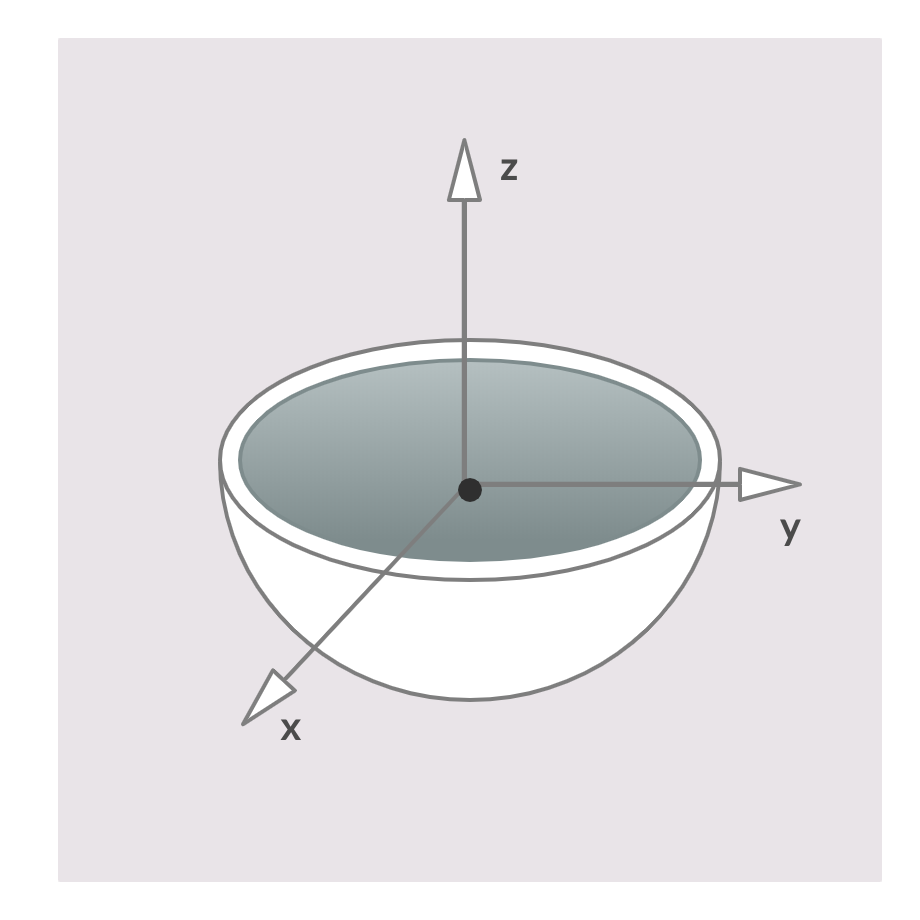
\includegraphics[width=0.8\linewidth]{halvkule.png}}
  \caption{
  Here you see the hemisphere shell. The origin is equidistant to the hemisphere and the hemisphere is oriented such that it has rotational symmetry along the z-axis. \label{fig:hemisphere}
  }
\end{figure}
%\clearpage % flush figures fig:hemisphere



\subex{a)}
Calculate the field in the origin.


% --- begin solution of exercise ---
\paragraph{Solution.}
Electric field from a small surface element is given by
\begin{equation}
d\mathbf{E} = \frac{1}{4\pi\epsilon_0}\frac{\rho}{R²}\hat{r}
\end{equation}
Where $\hat{r}$ is a unit vector pointing from the surface element to the origin. Notice that because the origin is equidistant to the hemisphere, the distance from any surface element to the origin is the same. Because of symmetry we only need to look at the component in z-direction (any x- and y-component cancel out). Therefore we get the following expression:
\begin{equation}
dE_z = d\mathbf{E}\cdot\hat{z} = \frac{1}{4\pi\epsilon_0}\frac{\rho}{R²}\hat{r} \cdot \hat{z} = \frac{1}{4\pi\epsilon_0}\frac{\rho}{R²}cos(\theta)
\end{equation}
Make sure you understand the last transition, if not; express $\hat{r}$ in spherical coordinates and then carry out the dot product. Because we are working with a spherical shape it can be a good idea to transition to spherical coordinates when we do the surface integral. Substituting $dS = R²sin(\theta)d\phi d\theta$ we get the following integral:
\begin{equation}
E_z = \frac{\rho}{4\pi \epsilon_0} \int_0^{2\pi}\int_0^{\pi/2}sin(\theta)cos(\theta)d\theta d\phi = \frac{\rho}{4\epsilon_0}
\end{equation}
Therefore we get the Field
\begin{equation}
\mathbf{E}_z = \frac{\rho}{4\epsilon_0}\hat{z}
\end{equation}

% --- end solution of exercise ---

\end{doconceexercise}
% --- end exercise ---


% ------------------- end of main content ---------------

% #ifdef PREAMBLE
\end{document}
% #endif

